% This is the Reed College LaTeX thesis template. Most of the work
% for the document class was done by Sam Noble (SN), as well as this
% template. Later comments etc. by Ben Salzberg (BTS). Additional
% restructuring and APA support by Jess Youngberg (JY).
% Your comments and suggestions are more than welcome; please email
% them to cus@reed.edu
%
% See http://web.reed.edu/cis/help/latex.html for help. There are a
% great bunch of help pages there, with notes on
% getting started, bibtex, etc. Go there and read it if you're not
% already familiar with LaTeX.
%
% Any line that starts with a percent symbol is a comment.
% They won't show up in the document, and are useful for notes
% to yourself and explaining commands.
% Commenting also removes a line from the document;
% very handy for troubleshooting problems. -BTS

% As far as I know, this follows the requirements laid out in
% the 2002-2003 Senior Handbook. Ask a librarian to check the
% document before binding. -SN

%%
%% Preamble
%%
% \documentclass{<something>} must begin each LaTeX document
\documentclass[12pt,twoside]{reedthesis}
% Packages are extensions to the basic LaTeX functions. Whatever you
% want to typeset, there is probably a package out there for it.
% Chemistry (chemtex), screenplays, you name it.
% Check out CTAN to see: http://www.ctan.org/
%%
\usepackage{graphicx,latexsym}
\usepackage{amsmath}
\usepackage{amssymb,amsthm}
\usepackage{longtable,booktabs,setspace}
\usepackage{chemarr} %% Useful for one reaction arrow, useless if you're not a chem major
\usepackage[hyphens]{url}
% Added by CII
\usepackage{hyperref}
\usepackage{lmodern}
\usepackage{float}
\floatplacement{figure}{H}
% End of CII addition
\usepackage{rotating}

% Next line commented out by CII
%%% \usepackage{natbib}
% Comment out the natbib line above and uncomment the following two lines to use the new
% biblatex-chicago style, for Chicago A. Also make some changes at the end where the
% bibliography is included.
%\usepackage{biblatex-chicago}
%\bibliography{thesis}


% Added by CII (Thanks, Hadley!)
% Use ref for internal links
\renewcommand{\hyperref}[2][???]{\autoref{#1}}
\def\chapterautorefname{Chapter}
\def\sectionautorefname{Section}
\def\subsectionautorefname{Subsection}
% End of CII addition

% Added by CII
\usepackage{caption}
\captionsetup{width=5in}
% End of CII addition

% \usepackage{times} % other fonts are available like times, bookman, charter, palatino


% To pass between YAML and LaTeX the dollar signs are added by CII
\title{A Big Data Analysis of Pokémon Battling}
\author{Samuel D. Olson}
% The month and year that you submit your FINAL draft TO THE LIBRARY (May or December)
\date{May 2017}
\division{Mathematics and Natural Sciences}
\advisor{Prof.~Bray}
%If you have two advisors for some reason, you can use the following
% Uncommented out by CII
\altadvisor{Prof.~Lau}
% End of CII addition

%%% Remember to use the correct department!
\department{Mathematics}
% if you're writing a thesis in an interdisciplinary major,
% uncomment the line below and change the text as appropriate.
% check the Senior Handbook if unsure.
%\thedivisionof{The Established Interdisciplinary Committee for}
% if you want the approval page to say "Approved for the Committee",
% uncomment the next line
%\approvedforthe{Committee}

% Added by CII
%%% Copied from knitr
%% maxwidth is the original width if it's less than linewidth
%% otherwise use linewidth (to make sure the graphics do not exceed the margin)
\makeatletter
\def\maxwidth{ %
  \ifdim\Gin@nat@width>\linewidth
    \linewidth
  \else
    \Gin@nat@width
  \fi
}
\makeatother

\renewcommand{\contentsname}{Table of Contents}
% End of CII addition

\setlength{\parskip}{0pt}

% Added by CII

\providecommand{\tightlist}{%
  \setlength{\itemsep}{0pt}\setlength{\parskip}{0pt}}

\Acknowledgements{
I wanted to thank everyone working for Pokémon Showdown for the
opportunity to work with a rich dataset that continues to pose
challenges well beyond the realm of Pokémon battling.
}

\Dedication{
This work is dedicated to all past, current and future members of The
Rocking Chair.
}

\Preface{
Overall, the this study highlights the gains to model quality when
including parameters of team composition rather than battle decisions.
Specifically in regards to Pokémon battling, the effectiveness of
utilizing entry hazards is considered. Some evidence is provided that
supports the statistical significance of using entry hazards, but the
variability between entry hazards is highlighted in greater detail.The
study lends support to the use of entry hazards as an effective Pokémon
battling strategy, while at the same time highlighting the limitations
of using the results prescriptively in a Pokémon battle.
}

\Abstract{
\par  

The study lends support to the use of entry hazards as an effective
Pokémon battling strategy, while at the same time highlighting the
limitations of using the results prescriptively in a Pokémon battle.
}

% End of CII addition
%%
%% End Preamble
%%
%

\begin{document}

% Everything below added by CII
      \maketitle
  
  \frontmatter % this stuff will be roman-numbered
  \pagestyle{empty} % this removes page numbers from the frontmatter

      \begin{acknowledgements}
      I wanted to thank everyone working for Pokémon Showdown for the
      opportunity to work with a rich dataset that continues to pose
      challenges well beyond the realm of Pokémon battling.
    \end{acknowledgements}
  
      \begin{preface}
      Overall, the this study highlights the gains to model quality when
      including parameters of team composition rather than battle decisions.
      Specifically in regards to Pokémon battling, the effectiveness of
      utilizing entry hazards is considered. Some evidence is provided that
      supports the statistical significance of using entry hazards, but the
      variability between entry hazards is highlighted in greater detail.The
      study lends support to the use of entry hazards as an effective Pokémon
      battling strategy, while at the same time highlighting the limitations
      of using the results prescriptively in a Pokémon battle.
    \end{preface}
  
      \hypersetup{linkcolor=black}
    \setcounter{tocdepth}{2}
    \tableofcontents
  
      \listoftables
  
      \listoffigures
  
      \begin{abstract}
      \par  
      
      The study lends support to the use of entry hazards as an effective
      Pokémon battling strategy, while at the same time highlighting the
      limitations of using the results prescriptively in a Pokémon battle.
    \end{abstract}
  
      \begin{dedication}
      This work is dedicated to all past, current and future members of The
      Rocking Chair.
    \end{dedication}
  
  \mainmatter % here the regular arabic numbering starts
  \pagestyle{fancyplain} % turns page numbering back on

  \chapter{Pokémon, Game Theory, and Behavioral Economics: A Brief
  Overview}\label{pokemon-game-theory-and-behavioral-economics-a-brief-overview}
  
  \section{Introduction}\label{introduction}
  
  The world of Pokémon began in 1995 with the pair of games Pokémon Red
  and Green. For Western audiences, the latter game would become known as
  Pokémon Blue. These two games introduced a unique system of turn-based
  that continues to define the franchise of Pokémon games. Numerous other
  games have attempted to copy the Pokémon battling format, but none have
  been able to equal its widespread appeal and dedicated player base. With
  each successive iteration, new items, Pokémon types, and of course new
  species of Pokémon are added to the Pokémon lexicon. As a result the
  world of Pokémon has continued to grow and evolve into one of the
  largest video games franchises to date. The most recent iteration of
  Pokémon games, Pokémon Sun and Moon, have continued Pokémon's commercial
  and historical trend of turning profits while adding layers to an
  already complex system of battling.
  
  Since 2011 the program Pokémon Showdown has offered a simplified version
  of Pokémon games. This simplified version allows players to exclusively
  battle one another, replicating the most recent iteration of the Pokémon
  games in the process. This has allowed players to hone and test their
  Pokémon battling skills through the years. With well-over 20,000 daily
  registered users and counting, this program has become the go-to program
  to test and practice Pokémon battling strategies in the ultimate pursuit
  of becoming the very best that no one ever was.
  
  However, before any formal analysis of Pokémon battling is discussed the
  battling system must be rigorously detailed for laymen and theorists
  alike.
  
  First and foremost, each Pokémon battle occurs exclusively between two
  players. Each of the two players has a team composed of six Pokémon. For
  the purposes of analysis teams with duplicate Pokémon will not be
  considered, namely because such teams are not allowed in ranked battles.
  As such, teams are composed of six distinct Pokémon. Depending on the
  battle format, the team of six Pokémon is either randomly assigned or
  dictated by the player. The two formats being considered in this study,
  random battles and overused, provide an example of each respectively. As
  a point of note, only battles in the `Anything Goes' category allow any
  Pokémon to be used, including duplicate species within a player's team.
  
  Regardless of the battle format, each turn each player simultaneously
  make a decision for the Pokémon they have on the field. The decisions
  are then executed. The order of play is decided by comparison of the
  selected moves. Priority is given first to priority moves and then, if
  neither player selected a priority move for the turn, by a comparative
  assessment of the two Pokémons' speeds.
  
  The potential moves Pokémon are able to execute have a wide variety of
  effects. This will be detailed later however. Regardless of the damage
  or effects of the executed moves, once a player's Pokémon loses all of
  its health, an event referred to as fainting, the player must switch
  into another Pokémon. If a player has no other Pokémon to switch into,
  the battle ends. As would be expected, the player whose Pokémon have all
  fainted loses the battle. Consequently the player who eliminates all of
  their opponent's Pokémon wins.
  
  Furthermore, each Pokémon has at most four possible moves to chose from
  during any turn of a battle. Whenever a player has at least two Pokémon
  that have not fainted, they have additional choice to switch into
  another Pokémon. Doing so counts as the player's action for the turn. As
  a result, players almost always have five different choices to make each
  turn.
  
  There are still a number of other details that are relevant to consider
  beyond those already mentioned. Namely, while some information is fixed
  during the battle -such as the opposing players team composition- some
  variables of interest are case-specific. These include what moves an
  opposing Pokémon has already used, and consequently revealed, along with
  a given Pokémon's held item, its ability, and a slew of other variables.
  However, similar to the different type of moves a Pokémon can chose
  from, these points will be detailed in the methodology section.
  
  That being said, to formally analyze Pokémon battling the game itself
  must be formally denoted in game theoretic terms. This will aid in both
  describing the game and in highlighting its complexity. With this in
  mind, it bears noting that there are only two outcomes to any battle:
  One player wins and the other loses. Because of this, Pokémon battling
  is by definition a zero-sum game. However, it is important to note that
  there some distinctions between how a player wins or loses a game.
  Though the game ends when all of the Pokémon on one team have fainted,
  any player has the choice to forfeit the game any time before this
  occurs. Thus, the two ways to win or lose a battle are either by
  forfeiture or by having all of their Pokémon faint; this latter outcome
  is referred to as a ``normal'' game. Additionally, there is the
  potential for a game to result in a draw. However, draws result in a
  neutral payoff as neither player raises or lowers their ranking after a
  draw.
  
  Within the scope of game theoretic terms, it is vital to note that each
  player is able to see all past decisions made over the course of a
  battle, and that battles typically last a number of turns. Speaking to
  the former point, players are able to recall not only their past
  decisions but also those of their opponent, including how much damage
  was done by a specific move during a previous turn. As this information
  is available at any time during the battle, Pokémon battling is a
  perfect recall game. Furthermore as each game is composed of a sequence
  of turns, Pokémon battling is also a sequential game.
  
  The points noted on information allude to a unique trait of Pokémon
  battling that further details the type of game Pokémon battling is: An
  incomplete information game. Though the extent of incompleteness is
  format specific, each player is given limited information about the
  opposing player's team at the beginning of the battle. After each turn,
  players learn not only the different moves each opposing Pokémon has,
  but also their abilities, held items, and sometimes what other Pokémon
  compose the opposing team. Generally speaking, there is almost always
  new information revealed each turn.
  
  However, the extent to which player strategies are revealed from
  revealed information is an open topic of discussion, both in this study
  and in current game theory literature. Naturally, the analysis of such a
  topic relies upon at least one apriori assumption, namely that player
  strategies are revealed by their past decisions. However, whether player
  strategies are rational and consistent is another matter entirely;
  nonetheless, it is important to note that incorporating such information
  into players own decision-making complicates analysis and is a central
  topic in analyzing Pokémon battling.
  
  Taken together, Pokémon battling is a special case of a sequential,
  zero-sum two-player game with incomplete information and perfect recall.
  As Pokémon battling lends itself to a discussion of imperfect
  information, it is all the more vital to consider the role of decision
  making within the context of sequential games. However, it is vital to
  note that this study will not do so using expansive game trees or
  comparison of payoffs. Namely this is done due to computational
  limitations.
  
  Game theoretics aside, there are also important computational notes to
  detail. In this regard, initial computations and analysis focus on the
  distributions of turn length, i.e.~the length of games played when one
  player forfeited or had all of their Pokémon faint and the corresponding
  distribution of game lengths. After these distributional computations, I
  categorize moves by their type, specifically whether a specific move is
  damaging or what is referred to as a ``setup'' move. After this
  categorization I gauge the effectiveness of using specific moves on the
  empirical probability that using such move corresponded to a winning
  outcome.
  
  Overall I explore the decision-making process involved in Pokémon
  battling. By incorporating tenants of behavioral economics and game
  theory, I hope to highlight not only the empirical probabilities of
  winning associated with specific move sets, but also analyze how and why
  such events occur. More specifically I will continue the recent trend of
  `Big Data' analysis to explore macro trends in player's decision making
  processes In doing so I hope to answer two main questions: What factors
  influence the liklihood of winning a Pokémon battle, and are these
  findings generalizable across specifications? In the context of Pokémon
  battling, is a player marginally better of by deciding to use one type
  of entry hazard over another?
  
  \section{Literature Review}\label{literature-review}
  
  Scant rigorous or academic research has been conducted within the scope
  of Pokémon-related topics. The most frequent publications have focused
  either on Pokémon as a cultural phenomena or have been official strategy
  guides for the various Pokémon games published by Nintendo affiliates.
  Importantly, these strategy guides do not detail Pokémon battling
  strategies, although they do detail the numerous Pokémon species, items,
  and moves available in each game. It comes as no surprise then that the
  Pokémon strategy guides do not formally detail Pokémon battling
  strategies or use of game theoretic terminology. That isn't to say that
  there aren't publications focusing on Pokémon battling strategies.
  
  Academic papers that focus Pokémon battling have developed and analyzed
  algorithms to simulate Pokémon battling and engage in Pokémon battling
  against human players in the program Pokémon Showdown. The first paper
  of this kind gives a rudimentary background on Pokémon battling and
  focuses explicitly on 1v1 battle simulations (Gildardo 2013). However,
  in a detailed analysis of one particular one-on-one scenario the author
  is singularly-minded, insomuch as literally focusing only on one-on-one
  Pokémon battles. Furthermore, Gildardo (2013) does not consider other
  potential variants on Pokémon abilities or item pairings. In this
  regard, Gildardo's article does not go into great detail on the many
  variants of Pokémon battling, as highlighted by the exclusion of teams
  of Pokémon.
  
  This point notwithstanding, since Gildardo (2013) there has been one
  other notable publication that focuses on Pokémon battling. This
  publication focuses on the creation and analysis of algorithms within
  the context of Pokémon battling; the article additionally goes into
  greater detail on battling strategies while incorporating comparative
  analysis of the different algorithms used to play against human
  opponents (Ho et al. 2016). Though Ho et al. 2016 focused on what is
  currently a previous iteration of Pokémon Showdown, the iteration of
  Pokémon Showdown is fundamentally the same as that of the data used in
  this study. Nonetheless, the paper did have its own shortcomings as
  well. Namely, the algorithms used would never select a move whose type
  would be not very effective against the opponents fielded Pokémon. This
  point will be detailed later, but needless to say such a decision is not
  always the preferred one.
  
  Furthermore, on the subject of different versions of Pokémon Showdown,
  relevant documentation of the past iterations of Pokémon Showdown are
  available at the program's website. The website for Pokémon Showdown
  provides a hub for information ranging from Pokémon battling basics to
  specific battle format descriptions. Similar to all information
  mentioned thus far, replays and ladder ranking are available publically.
  Furthermore the site provides Pokémon usage statistics and a damage
  calculator for aspiring Pokémon battlers.
  
  As noted previously, game theory vernacular has not entered into
  discussions on Pokémon battling strategies, at least in any formal
  setting. Applying such concepts to the context of Pokémon battling
  offers a formal foundation to discuss strategies and test hypotheses. In
  this regard, there are three main areas of game theory that intersect in
  the analysis of Pokémon battling. These three areas of interest include
  the interpretation of Pokémon battling as a zero sum game, the role of
  incomplete information, and the implications of Pokémon battling as a
  non-cooperative game. These three topics actively influence the
  decision-making process associated with Pokémon battling.
  
  A central factor involved in the decision making process as it relates
  to game theory is the role of information, specifically how players
  incorporate information revealed each turn into their strategies. As
  information is revealed each turn, including the four moves an opposing
  Pokémon has, its ability, held item, along with what other Pokémon are
  on the opposing team, it is vital for players to determine if the
  information they just received is relevant. Furthermore, players need to
  decide if the information provides any insight into their opponent's
  strategy. Overall, this speaks to Pokémon not being a perfect
  information game. As such, it is not possible to apply Zermelo's
  theorem, though its negation provides insight as to the possible
  existence of a winning strategy (Schwalbe et al. 2001).
  
  An especially interesting addition to the analysis of incomplete
  information in Pokémon battling is the topic and implications of
  asymmetrical information. In this regard, the concepts of sunk costs and
  signaling may enter into the equation. Especially for the Random battle
  format, each player is given minimal information at the onset of the
  game. And while each turn, players both gain information, they may
  receive new information at different rates. The implications of this
  point may provide insight into specific strategies, and is a point of
  future analysis.
  
  This being said, concepts from game theory are not the only relevant
  ideas for analyzing Pokémon battling. In the context of exploring the
  frequency of players switching Pokémon will necessarily invoke concepts
  from from behavioral economics as well as game theory. Relevant to the
  field of behavioral economics, the concept of ``keeping doors open''
  applies as well as post-op payoff analysis. The concept of ``keeping
  doors'' open is explored in Chapter 6 of Ariely's work Predictably
  Irrational, giving a semblence of what the expected results may be. In
  the context of Pokémon battling, players may decide to preemptively
  switch Pokémon in the hopes of having that Pokémon later in the battle.
  Via application of Ariely's empirical results players may prefer to keep
  options -availability of certain Pokémon- open, even if doing so incurs
  costs and/or reduces their chances of winning. Whether this adversely
  influences the players' outcomes is another point of inquiry.
  
  \chapter{Methodology}\label{methodology}
  
  The data used is a compilation of battle logs taken from the Pokémon
  Showdown servers. Each battle log is stored as a .json file. The data
  spans the entirety of December 25th, 2015. No battle logs are
  incomplete, i.e.~none of the daily data entries are empty, though some
  are excluded for reasons covered later. Overall, there were no dramatic
  overhauls done to Pokémon battling formats or the overall system for the
  data used in this study. However, some adjustments have been made since
  the time covered in this study and will be highlighted in the analysis
  portion of the study.
  
  Furthermore only ranked games are included in the dataset. Ranked
  battles are battles that count towards a players global ranking in
  Pokémon Showdown. For each battle, players stand to gain or lose ranking
  points depending on whether they win or lose the battle. A number of
  links redirect users to the host site of this game: Smogon University.
  This website offers a wide variety of resources, similar to those found
  at the Pokémon Showdown website. Most importantly the Smogon forums are
  a prominent site for discussion of Pokémon battling strategies.
  
  \section{Pokémon Battling Basics}\label{pokemon-battling-basics}
  
  The Pokémon battle starts with Pokémon being sent out. For the purposes
  of the data used, one Pokémon is sent out for each opponent, totalling
  two Pokémon being out at any given time. Following this, each Pokémon
  has 4 moves to choose from, along with the option to switch to a
  different Pokémon (when applicable). After both players make a decision,
  the moves are weighted for priority and speed to determine the order of
  play. If both players decide not to switch one Pokémon will attack the
  other, after which the next Pokémon will do the same if it has not
  fainted. After each move has been executed the turn ends and the process
  is repeated. When one of the Pokémon faints, the player whose Pokémon
  fainted will be prompted to select another Pokémon from the bench. The
  first player to lose all of their Pokémon loses the battle.
  
  However, before the nitty gritty details are explained it is important
  to make a concession. The entirety of the Pokémon battling system- even
  that used in the data -is not included in this analysis. The number of
  cases that deviate from the rules detailed below are either not included
  in the competitive format, or are generally inconsequential to the
  scenarios and strategies considered in this study.
  
  \subsection{Battle Formats}\label{battle-formats}
  
  The data used for this study includes only one battling format. The two
  most frequently used formats are known as Over Used and Random Battles,
  abbreviated as OU and Randbats respectively. Both formats have teams of
  six Pokémon and only allow one Pokémon to be out at any given time.
  While both battle formats are subsets of what are known as single
  battles, only OU will be highlighted in greater detail.
  
  The OU format includes team composition. By including team composition,
  players are able to decide what Pokémon to include on their team, the
  moves of each Pokémon, and other factors such as held items and
  abilities. However, there are still some restrictions placed on players.
  Specific species of Pokémon are barred from use, notably Pokémon
  classified as ``Ubers'' that include a large portion of legendary and
  mega-Pokémon. Additionally certain ``hidden'' abilities are restricted,
  limiting the possible Pokémon abilities a specific species may use for a
  given format.
  
  \subsection{Pokémon Types}\label{pokemon-types}
  
  Typeage is a unique characteristic to Pokémon battling. Currently there
  are 18 distinct types. These include normal, fire, water, electric,
  grass, ice, fighting, poison, ground, flying, psychic, bug, rock, ghost,
  dragon, dark, steel, and fairy. Both moves and Pokémon are given a type
  attribute, though moves are only one type. And While a move may only be
  one of the 18 types, a Pokémon can be at most two different types at
  once.
  
  However, some of these combinations are not found in Pokémon. From the
  initially possible 171 Pokémon type combinations, 18 choose 2 plus 18
  monotypes, there are actually only 133 types that a players may
  encounter or chose from (as 38 type combinations had not yet been used
  during 2015). It is also worth noting that some Pokémon are able to
  change type during a battle, but for the purposes of analysis these
  Pokémon will be considered after-the-fact.
  
  The typeage of each Pokémon influence not only the potential weaknesses
  of each Pokémon, but also the amount of damage that type-specific moves
  are able to do. Each Pokémon has at least one and at most two types. If
  a Pokémon uses a damaging move whose type corresponds to type of the
  Pokémon that used it, that Pokémon gets a same type attack bonus,
  abbreviated as a ``stab'' bonus. This causes the move to do 50\% more
  damage, potentially 100\% if the Pokémon also has the ability
  Adaptability.
  
  \subsection{Pokémon Attributes}\label{pokemon-attributes}
  
  Generally, there are a number of factors that are specific to each
  Pokémon. Some of these factors are considered static, meaning that they
  do not and cannot change over the course of the battle. These types of
  factors are defined as ``Fixed'' attributes. However some factors -such
  as the stats of a Pokémon- that are fixed at the beginning of the battle
  \emph{can} change over the course of a battle. There are also a number
  of factors that are able to generally change over the course of a
  battle. Such factors, by constrast, are defined as ``Variable''
  attributes. The terminology is largely taken from Ho et al. for ease of
  translation and applicability. The attributes are detailed in the order
  given.
  
  \subsection{Pokémon Fixed Attributes}\label{pokemon-fixed-attributes}
  
  Fixed attributes include the typeage of a Pokémon, the four moves each
  specie Pokémon has, the item the Pokémon holds, the Pokémon's ability,
  the level of the Pokémon, and the Pokémon's baseline stats. However,
  there are exceptions to the rules for each of these attributes except
  for the level of the Pokémon. Every fixed attribute and its respective
  exception(s) will be considered in order.
  
  First and foremost is the typeage of a Pokémon, detailed previously.
  However, one possible method for a Pokémon to change its type is
  specific to a Pokémon's ability. Both Protean and Color Change are
  abilities that are able to change a friendly Pokémon's typeage. The
  former ability changes the Pokémon Kecleon's type to that of the move
  that affected it, whereas the latter ability turns its type into the
  typeage of the move that just was just used by the Pokémon Greninja.
  These two abilities are specific to Kecleon and Greninja specifically.
  Furthermore, there are moves that able to make the opponents Pokémon
  into a water, grass, or ghost Pokémon -on top of their previous typeage-
  if they use the moves soak, forest's curse, and treat-or-treat
  respectively.
  
  Each Pokémon's set moves are also fixed during a battle. The exception
  to this occurs when a Pokémon runs out of power points -denoted as PP-
  for all of its four moves, at which point it is only able to use the
  move struggle. Every move has a set limit to the number of times it can
  be used, though the number of times a move can be used varies across the
  set of moves. The struggle is real.
  
  Pokémon are able to hold one item at the beginning of the match. Pokémon
  may also lose their held item either by being hit by the move Knock-off,
  which knocks the opponent's Pokémon's item off, or by using their held
  item. Held items are able to be consumed for a one-time effect. This
  scenario often includes the consumption of berries, which offer a
  variety of different effects to the Pokémon holding it. For example, if
  a Pokémon is given a status condition -a condition detailed in the
  following section- from an opposing Pokémon while holding a Lum berry,
  the berry will be consumed and the Pokémon's status condition will be
  cured. This example highlights an important characteristic of some
  held-items: Some items may only be used once and are discarded after
  their initial use.
  
  One of the most important items that a Pokémon can hold is an item that
  allows the Pokémon to Mega-Evolve, increasing its stats, changing its
  ability, and even changing the typeage of the Pokémon. This special case
  of item holding is a focus of this study. Additionally, only one
  Mega-Pokémon is allowed on a team at once, making variables that account
  for the different Mega-Pokémon independent by nature.
  
  Similar to items, a Pokémon can only have one ability at a time.
  However, by contrast to a Pokémon's held item a Pokémon always has an
  ability. Nonetheless, Pokémon may have their ability swapped with
  another Pokémon's. This scenario only occurs a Pokémon makes physical
  contact with Yamask or Cofagrigus, at which point its ability is swapped
  with Mummy. Mummy will only change a physically-attacking Pokémon's
  ability; it has no other effect.
  
  The level of a Pokémon varies between one and one-hundred. The higher
  the level, the better the baseline stats for a given Pokémon,
  specifically in comparison to lower levels of that given Pokémon.
  Baseline stats are divided into six categories. These categories include
  (baseline) health, attack, special attack, defense, special defense, and
  speed. There is further nuance with the inclusion of Pokémon natures and
  Individual Values, or IVs. These factors influence the base stats of
  each Pokémon. However due to the sheer number of trivial combinations of
  IV spreads and nature choices, these two factors will not be a pivotal
  aspect to the framework and analysis of Pokémon battling. Nonetheless,
  the votatility of these baseline stats will be considered as a variable
  attribute.
  
  \subsection{Pokémon Variable
  Attributes}\label{pokemon-variable-attributes}
  
  Variable Attributes include boosts or reductions to a Pokémon's baseline
  stats, the status condition of the Pokémon, the volatile status of the
  Pokémon, the current health of the Pokémon, and whether the Pokémon is
  currently active.
  
  The former-most attribute directly influences how effective an active
  Pokémon is able to be in battle. Pokémon are able to learn and use moves
  that can boost their own status or ones that reduce their opponents.
  However, these moves are only able to influence a Pokémon's attack,
  special attack, defense, special defense, or speed. For example, the
  move Swords Dance raises its users attack status so long as the Pokémon
  remains active. The move may be used multiple times, but is only
  effective until it boosts or lowers its target's baseline stat by 3 or
  1/3 respectively.
  
  Status conditions are composed of a variety of statuses. Pokémon that
  suffer a status condition are either burned, frozen, paralyzed,
  poisoned, badly poisoned, or have fallen asleep. A Pokémon can only
  suffer from one status condition at a time, although a Pokémon can
  suffer from multiple status conditions if it overcomes the first
  condition. Each of these statuses is distinct, though there are
  similarities between being poisoned or badly poisoned. A Pokémon that is
  just poisoned will take damage equal to 1/8th of its maximum HP at the
  end of each turn. By comparison a Pokémon that is badly poisoned takes
  n/16th of its maximum HP at the end of the nth turn the Pokémon has been
  badly poisoned. A Pokémon that is poison-type or steel-type is unable to
  be poisoned in any form, and if a Pokémon has the ability Poison Heal it
  is healed 1/8th of its maximum HP at the end of each turn.
  
  Is a Pokémon is burned it takes 1/8th of its maximum HP in damage at the
  end of the turn. This has recently been changed to 1/16th of its maximum
  HP per turn, but this is just a passing point of note. Regardless of the
  amount of damage done to the burned Pokémon, the burned Pokémon's
  physical attacks do half damage. The exception to this rule is if the
  affected Pokémon has the ability Guts. A fire-type Pokémon cannot be
  burned.
  
  In a similar vein to being burned, a paralyzed Pokémon has its speed
  reduced to 1/4th of its baseline speed. Furthermore, a Pokémon that is
  paralyzed has a 1/4 chance of not being able to move during its move.
  This event is referred to as being ``fully paralyzed''. Furthermore,
  electric-type Pokémon are unable to be paralyzed, and if a Pokémon has
  the ability Lightning Rod it's special attack is boosted by 1.5 its base
  level. Additionally, ground-type Pokémon cannot be paralyzed, just as
  they are not affected by electric-type moves.
  
  A Pokémon that has fallen asleep is unable to use its moves except for
  the moves Snore and Sleep Talk. A Pokémon falls asleep for one to five
  turns. However, if a Pokémon purposely puts itself to sleep using the
  move rest, it is asleep for exactly two turns. If a Pokémon has either
  of the abilities Vital Spirit or Insomnia it cannot be put to sleep.
  
  Lastly, there is the status condition of being frozen. Similar to
  previous typed statuses, ice type Pokémon are immune to becoming frozen,
  as are Pokémon with the ability Magma Armor. There is no set number of
  turns that a Pokémon can be frozen, but if a frozen Pokémon is hit by
  fire-type moves or the move scald is thaws out and is no longer frozen.
  
  Volative statuses are similar to status conditions, except that the
  volatile status will be negated by switching out the affected Pokémon,
  if applicable. Similar to status conditions, a Pokémon can only be
  affected by one volatile status at a time. Another important point to
  consider is that a Pokémon can suffer from both a volatile status
  \emph{and} a status condition. That being said, the most common form of
  volatile status is confusion. A Pokémon is confused for one to four
  turns, during which time the confused Pokémon has a 50\% chance to hurt
  itself instead of executing its move for the turn. A Pokémon may also be
  encored, meaning that it has to use the same move it just moved for 3
  turns. Additionally a Pokémon may flinch if hit before executing its
  move for the turn.
  
  Only currently active Pokémon are able to execute moves. Likewise, only
  active Pokémon may be damaged. Beyond this there is not anything else to
  detail in regards to the current health and activity of a Pokémon that
  is exclusive to variable attributes.
  
  \subsection{Environmental Variables}\label{environmental-variables}
  
  There are one class category to detail that is relevant to the analysis
  of Pokémon battling This category is the role of the environment in
  battling and is a central focus of the analysis of Pokémon battling.
  Though related to the different types of moves and abilities a Pokémon
  has, including both fixed and variable attributes, the environment is
  not specific to any one move, ability, or specie of Pokémon and as such
  must be highlighted separately from the previous attributions.
  
  The most prominent environmental variables to consider are what are
  referred to as ``set-up'' moves. These moves include Stealth Rock,
  Spikes, Toxic Spikes, Sticky Web, Light Screen, and Reflect. The latter
  two are different from the rest of the set-up moves in that they only
  last five turns, eight is the user was holding Light Clay when the move
  was used. When these moves are employed, the active Pokémon's special
  defense and defense are raised by one stage -or is increased by 1.5-
  respectively between Light Screen and Reflect.
  
  The former four set-up moves are a focal point of analysis and are in a
  category of moves known as entry hazard moves. These moves are of
  particular note because they can last for the entirety of a given
  battle. Once these moves are used, only certain moves or switches are
  able to eliminate them. Generally, using the move rapid spin or defog
  will eliminate the entry hazards, along with causing other effects.
  However, if a Pokémon uses defog both their and their opponents entry
  hazards will be eliminated, whereas rapid spin only eliminates entry
  hazards affecting the users team.
  
  Both Stealth Rock and Sticky Web can only be active once during a battle
  -unless previous uses of either are eliminated by methods previously
  noted. However, each have dramatically different effects. Specific to
  the latter, Pokémon that enter the field after Sticky Web is employed
  have their speed lowered by one stage -or 2/3rd their baseline level.
  This only applied to grounded Pokémon however, or non-flying type
  Pokémon. By contrast, Stealth Rock will damage any Pokémon that enters
  the field after it is used. The amount of damage done to the Pokémon
  depends on the type effectiveness of rock-type moves, as Stealth Rock is
  a rock-type move. In ascending order, Stealth Rock will do 3.125\%,
  6.25\%, 12.5\%, 25\%, and 50\% of the affected Pokémon's maximum health
  for type effectivenesses of 0.25x, 0.5x, 1x, 2x, and 4x respectively.
  
  Similar to Sticky Web, spikes only affect non-flying type Pokémon.
  However, spikes will inflict damage to Pokémon that switch in instead of
  afflicting them with a volatile or status condition. The amount of
  damage is dependent upon the number of layers of spikes active on the
  field. Spikes may be applied a maximum of three times. One layer of
  spikes will damage the opposing Pokémon by 1/8th of its maximum HP,
  while two layers will deal 1/6th, and three layers will do 1/4th of the
  opposing Pokémon's maximum health.
  
  Lastly is toxic spikes that, just like spikes and sticky web, only
  affect grounded Pokémon. However, toxic spikes are able to be applied
  two times. The first layer of toxic spikes will poison opposing Pokémon
  that switch in, while two layers of toxic spikes will badly poison
  Pokémon that switch in (that is if the Pokémon that switches in is able
  to be poisoned). Just like most other entry hazards, toxic spikes only
  affects grounded Pokémon.
  
  \section{Model Specification}\label{model-specification}
  
  As Pokémon battles have only two outcomes, we may estimate the
  probability of winning using a standard probit model. Let Y denote the
  outcome of any battle for a given player. Y takes the value of 0 if the
  player loses the battle and 1 if the player wins. To address the
  question of whether any entry hazards positively impact a player's
  liklihood of winning, we develop a number of different binomial probit
  models. Beginning with whether a specific move was used by a player in a
  battle, let the ith move be denoted \(M_i\). For models with entry
  hazards only, we have \(i=1,..4\). But over all models tested
  \(i=1,...,9\) to include moves that are able to supplement or supplant
  entry hazards. Similarly, we denote the jth Pokémon as \(P_j\), where
  \(j=1,...,415\). Furthermore, there are 39 different Mega-Pokémon that
  are usable in the OU format, so we denote the usage of the kth
  Mega-Pokémon as \(Mp_k\). In later model specifications, specific moves
  will be interacted with Pokémon selections. As an example, the
  specification of the model for the move stealth rock would include the
  full roster of moves and Pokémon, or
  \(\sum_{i=1}^{9} M_i + \sum_{j=1}^{415} P_j\) along with an interaction
  of each Pokémon that can potentially learn that move with the count of
  stealth rocks for that battle. The lth Pokémon that can learn Stealth
  Rock is denoted \(stP_l\). Similar notation is used for other
  move-specific Pokémon subsets.
  
  Letting \(\epsilon\) denote the error term, we begin with the simplified
  model. This model only includes whether a specific move was used. We
  have: \[(1): Y = \alpha + \sum_{i=1}^{9} M_i + \epsilon \] However, the
  repeated use of a move can lead to additional benefits. It is possible
  that the repeated use of a move has a lower marginal impact on a
  player's win liklihood. To test this hypothesis, we expand the initial
  model to include squared terms for each move. Thus we have:
  \[(2): Y = \alpha + \sum_{i=1}^{9} M_i + \sum_{i=1}^{9} M_i^2 + \epsilon \]
  
  These models have not yet included the vast variety of species composing
  teams. However, before examining the interactions between a team's
  composition of Pokémon and specific moves, there needs to be a formal
  model of just the marginal impact of a single Pokémon on a team.
  Respective to the indexing outlined previously, we have:
  \[(3): Y = \alpha + \sum_{j=1}^{415} P_j + \epsilon \] Thirty eight
  different Pokémon can turn into Mega-Pokémon however. To test whether a
  Pokémon negatively or positively impacts the marginal probability of
  winning, the next model specification includes Mega-Pokémon within the
  roster of competitive Pokémon.
  \[(4): Y = \alpha + \sum_{j=1}^{415} P_j + \sum_{k=1}^{39} Mp_k + \epsilon \]
  The next specification is the combination of models (1) and (4). Then,
  the last specification includes the interaction of having a specific
  Pokémon with the use of the move stealth rock. Respectively, the models
  are given by:
  \[(5): Y = \alpha + \sum_{i=1}^{9} M_i + \sum_{j=1}^{415} P_j + \sum_{k=1}^{39} Mp_k + \epsilon \]
  \[(6): Y = \alpha + \sum_{i=1}^{9} M_i + \sum_{j=1}^{415} P_j + \sum_{l=1}^{93} (M_1)*(stP_l)+ \sum_{k=1}^{39} Mp_k + \epsilon (6)\]
  
  After these six model specifications, the combination of all six models
  will be given to cross-check results and check for potential robustness
  for move and Pokémon combinations. The inclusion of interactions may be
  particularly key in identifying outlying results.
  
  \chapter{Data}\label{data}
  
  Due to the vast number of parameters included in the numerous models
  outlined previously, summary statistics and an output of five of the six
  models is contained in the Appendix section. Comments on each are
  provided with some brief context of their interpretation.
  
  Going in the order of the Appendices, the summary of the variables used
  in the analysis are a good starting point. The average game length is
  sixteen turns. However, the average is biased from games that lasted
  zero turns. As these games did not provide any meaningful information,
  they are excluded from all regressions used. Furthermore, in regards to
  ranking, most observations are within the range of 1000 to 1280 elo, as
  the mean rank is 1154 with a standard deviation of nearly 130 elo
  points. Given that the highest rank observed in the data is 1815, there
  is a noticeable divide between the highest ranking games and those
  within the range of standard deviations to the mean rank.
  
  Nonetheless, the real meat of the summary statistics is with the large
  range of different Pokémon species and Mega-Pokémon that players used.
  In this regard, nearly half of the most frequently used Pokémon, that of
  Alakazam, Banette, and Garchomp, have a Mega-evolution. Though
  specifically in regards to the Mega-evolution usage statistics, the four
  most frequently used Mega-Pokémon are Mega-Venusaur, Mega-Scizor, and
  both Mega-evolutions of Charizard, though Alakazam, Banette, and
  Garchomp are not the most infrequently used Mega-evolutions.
  
  It is important to bear in mind that Mega-Pokémon are not always
  utilized however, given by the fact that the cumulative sum of the mean
  of all Mega-Pokémon variables does not add up to one. Given this
  discrepancy, it would be fruitful to test whether utilizing a
  Mega-Pokémon marginally impacts whether a player wins a battle. Within
  this group of three Garchomp is the outlier, as both Mega-Alakazam and
  Mega-Banette were banned from the OU format following the year of the
  data used. Besides this standout feature of the summary statistics, the
  remaining frequently used Pokémon are considered staples of the OU
  format: Clefable, Talonflame, and Heatran. Of the total six most
  frequently used Pokémon, half have the ability to use the move Stealth
  Rock. This is important to bear in mind when considering the preliminary
  models.
  
  \begin{center}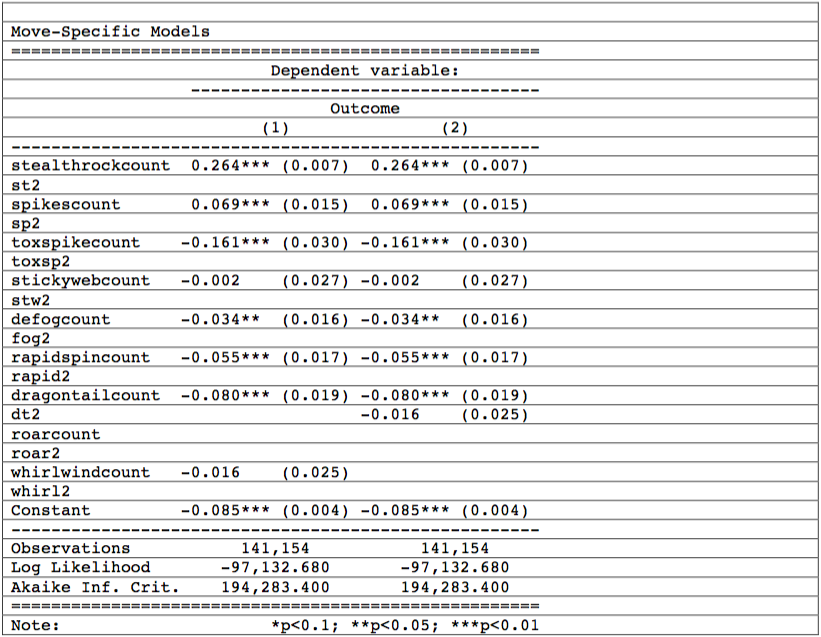
\includegraphics[width=400px]{table12} \end{center}
  
  Included above is the results of the first two model specifications.
  Sadly, the two models are alike in their log liklihood values and in
  their Akaike information criterion (AIC) values. Simply put, adding
  squared terms for the nine specified moves did not add anything
  meaningful to the initial model. This may be just a byproduct of the
  data however, as the only move variable with values greater than one was
  for the move Dragon Tail. Nonetheless, it is important to note that
  nearly all of the entry hazard moves are statistically significant.
  Though, this being said, only Stealth Rock and Spikes contribute
  positively to the marginal likliehood of winning a battle. This
  contributes to some semblence of generalizability though, as both
  Stealth Rock and Spikes are the only entry hazards that directly damage
  opposing Pokémon when they enter the battlefield.
  
  The statistical significance of the entry hazards is also verified in
  further model specifications. While the use of Toxic Spikes becomes less
  statistically significant with the inclusion of both single Pokémon
  choice and Mega-Pokémon choice, the sign of the variable remains
  negative. Furthermore, while later specifications continue to report
  Spikes as a statistically significant move choice, the magnitude of
  using the move appears to diminish when including other factors such as
  Pokémon choice.
  
  Overall, the use of Pokémon roster and Mega-Pokémon roster appear to be
  more meaningful variables than the use of simple move counts, as is
  evidence from comparison of log liklihood and AIC values. This
  improvement in model quality is also found in comparison to all previous
  models with the final model (6). While residual deviance is not reported
  for each model, the AIC lends credence to the comparative view of model
  (6) as the model of best fit for those specified. Though, this being
  said, the final model is particularly difficult to digest due to the
  number of parameters specified.
  
  The final model is adds meaningful insight to the simple move counting
  variables. Interacting the move count variable for Stealth Rock and all
  Pokémon that can potentially learn (and use) Stealth Rock, the model
  indicates that there is a nonuniform effect on win outcome depending on
  which Pokémon used it. This view may be appear counterintuitive, but it
  does offer a useful illustration to the complexity of Pokémon. Take for
  example two hypothetical instances where Stealth Rock is used by two
  different Pokémon on the same enemy Pokémon. While each may successfully
  execute the move on that turn, the opposing Pokémon gets to execute a
  move as well. If, in this instance, the move is the same, then damage is
  calculated according to the type matchup of the opposing move with the
  Pokémon; this may knock out one Pokémon while leave another with enough
  health to execute one more move.
  
  \chapter{Conclusion}\label{conclusion}
  
  Overall, the models improved in quality when more parameters were added.
  Additionally, including the interaction between using a specified move,
  Stealth Rock, and the inclusion of a specific Pokémon provided a more
  meaningful estimation of a player's liklihood to win a Pokémon battle.
  Overall, only one of the four entry hazards was not statistically
  significant across any model specifications. There is some evidence to
  support variability between different entry hazards, and the use of the
  moves Stealth Rock and Spikes contributed a positive marginal effect on
  a player's game outcome.
  
  Nonetheless, there are a number of other points to bear in mind. For
  starters, interactions were only considered between a move and a
  Pokémon, not one move and another move. This means that only the
  marginal effect of using Stealth Rock or Spikes was considered, not the
  joint use of Stealth Rock and Spikes. Furthermore, while ranking was
  briefly touched upon, no comparisons were made between different groups
  on the basis of rank. It would be meaningful to see if the usefulness of
  entry hazards was extended to groups that are considered high ranking,
  though this would significantly reduce the number of observations drawn
  upon.
  
  In regards to the missed opportunities associated with different
  interactions, there is one other elephant in the room: the Pokémon
  variables. While the models indicate whether one Pokémon has more wins
  or loses associated with its use, this is only a marginal effect being
  captured. Just as moves may interact or compound with the use of another
  move, so too can Pokémon. While including all combinations of six
  Pokémon would exhaust the degrees of freedom for the sample used,
  reducing the model to all combinations found in the sample would lend
  the data for more prescriptive use.
  
  Additionally, only one Pokémon battling format is considered during the
  study. Just as it would be intriging to see differences across rank,
  differences across battle format would lend greater external validity to
  the results found.
  
  \appendix
  
  \chapter{Appendix A: Summary
  Statistics}\label{appendix-a-summary-statistics}
  
  \begin{center}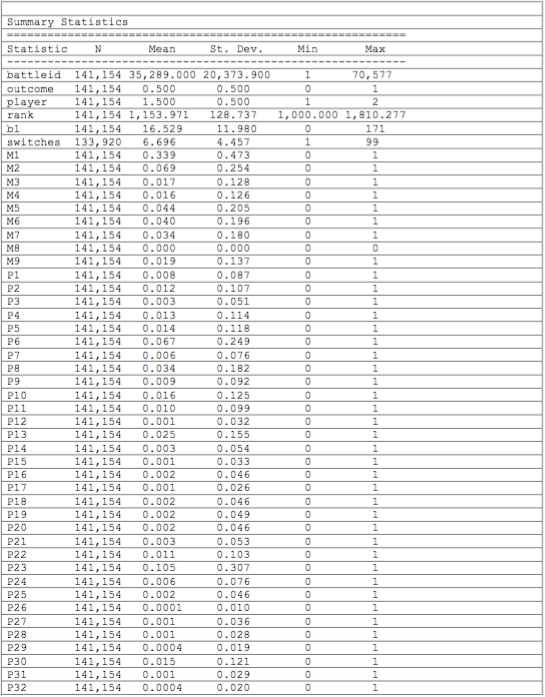
\includegraphics[width=400px]{t11} \end{center}
  
  \begin{center}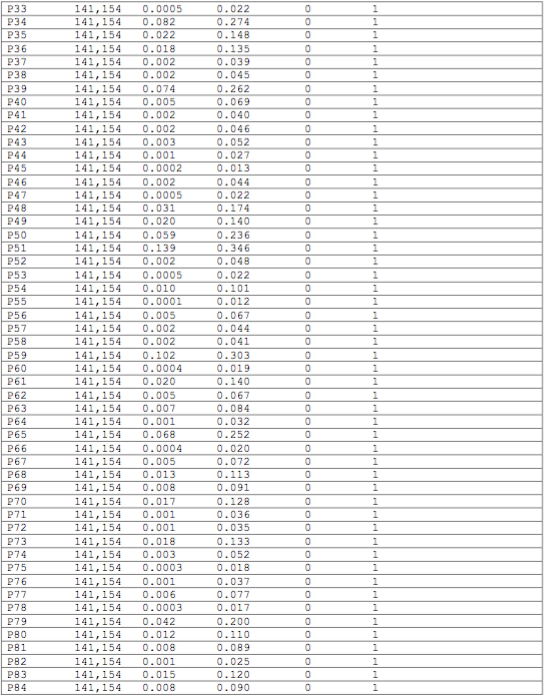
\includegraphics[width=400px]{t12} \end{center}
  
  \begin{center}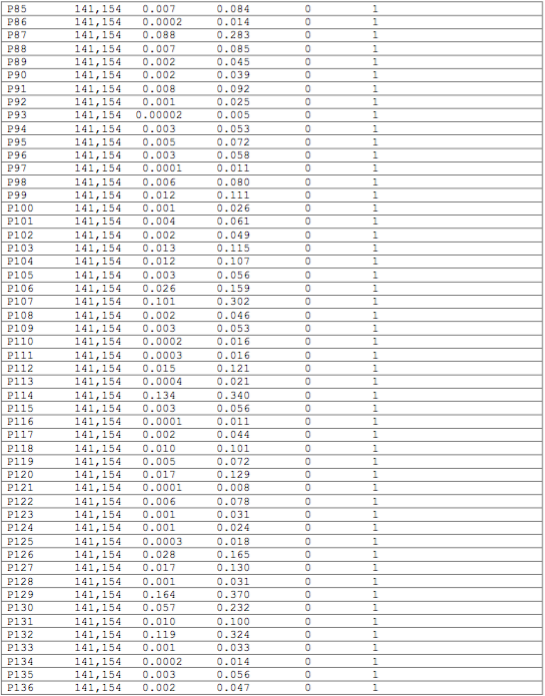
\includegraphics[width=400px]{t13} \end{center}
  
  \begin{center}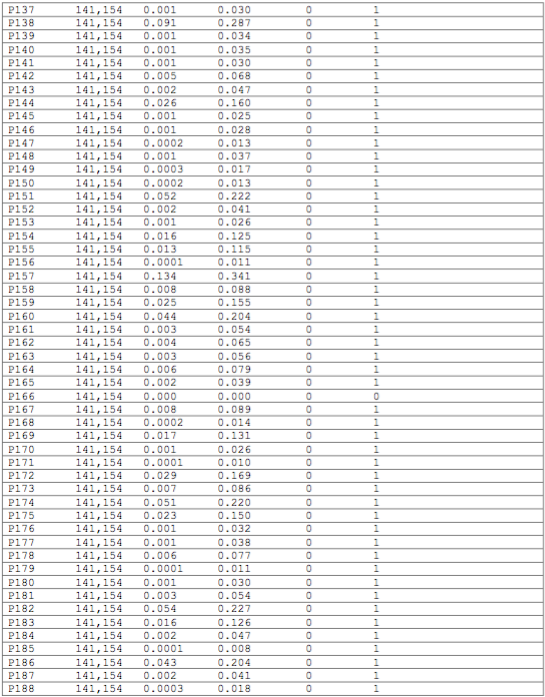
\includegraphics[width=400px]{t14} \end{center}
  
  \begin{center}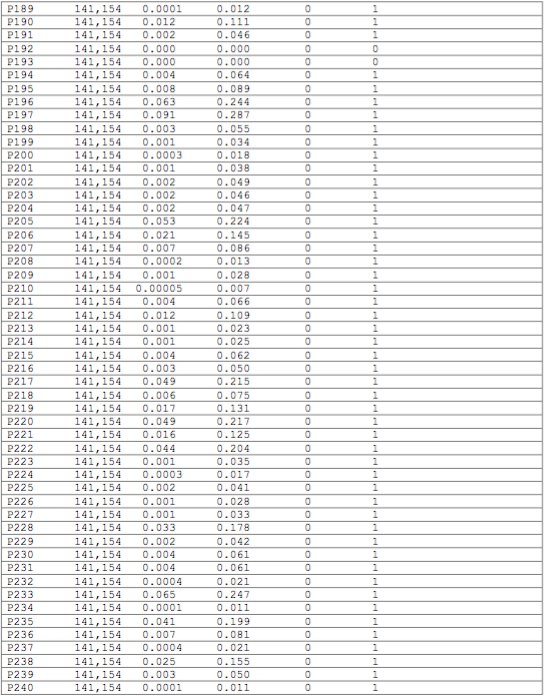
\includegraphics[width=400px]{t15} \end{center}
  
  \begin{center}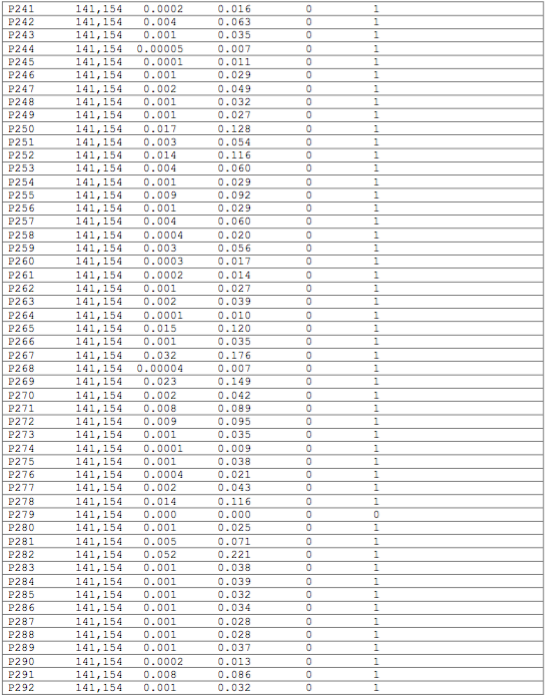
\includegraphics[width=400px]{t16} \end{center}
  
  \begin{center}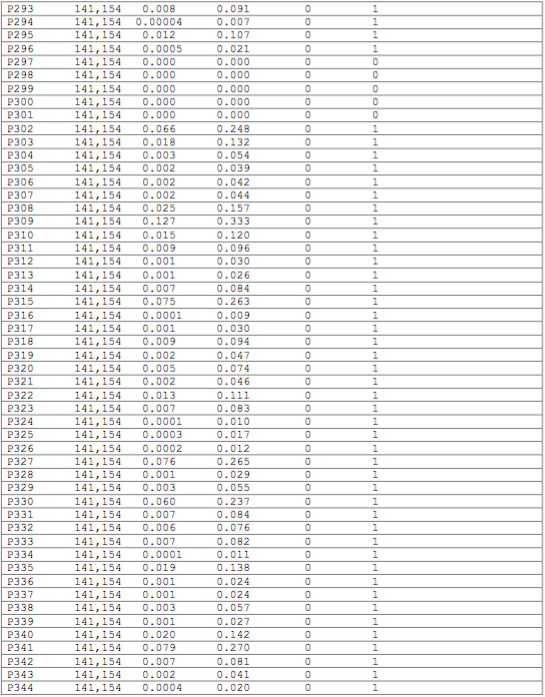
\includegraphics[width=400px]{t17} \end{center}
  
  \begin{center}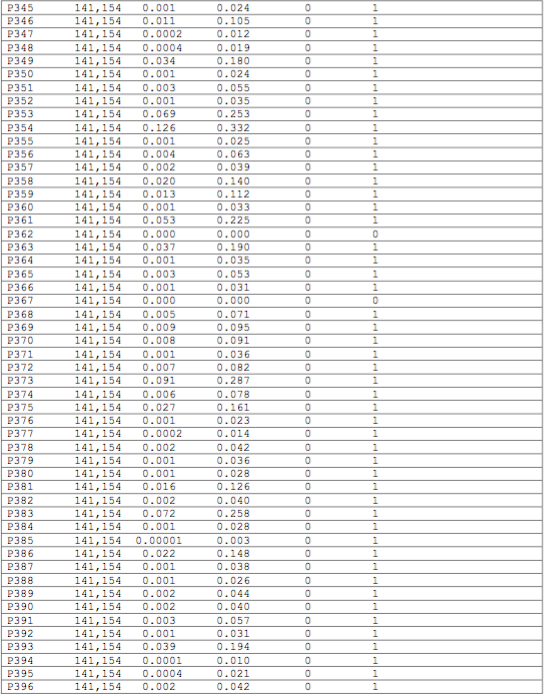
\includegraphics[width=400px]{t18} \end{center}
  
  \begin{center}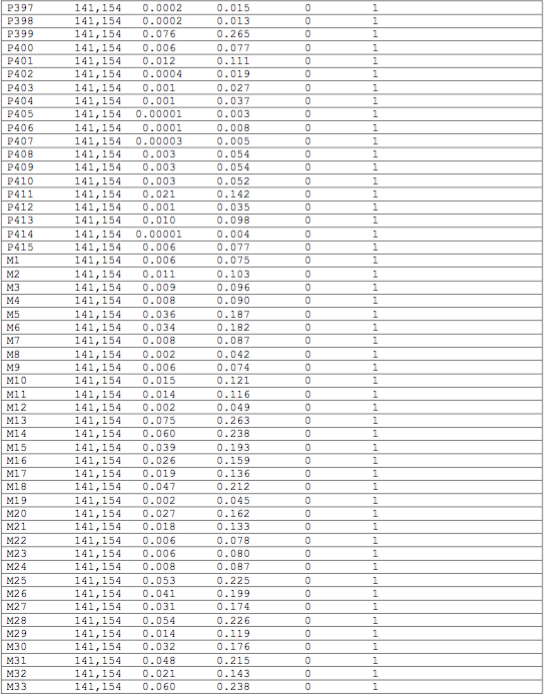
\includegraphics[width=400px]{t19} \end{center}
  
  \begin{center}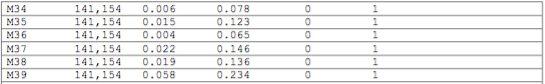
\includegraphics[width=400px]{t20} \end{center}
  
  \chapter{Appendix B: Model Summary}\label{appendix-b-model-summary}
  
  \begin{center}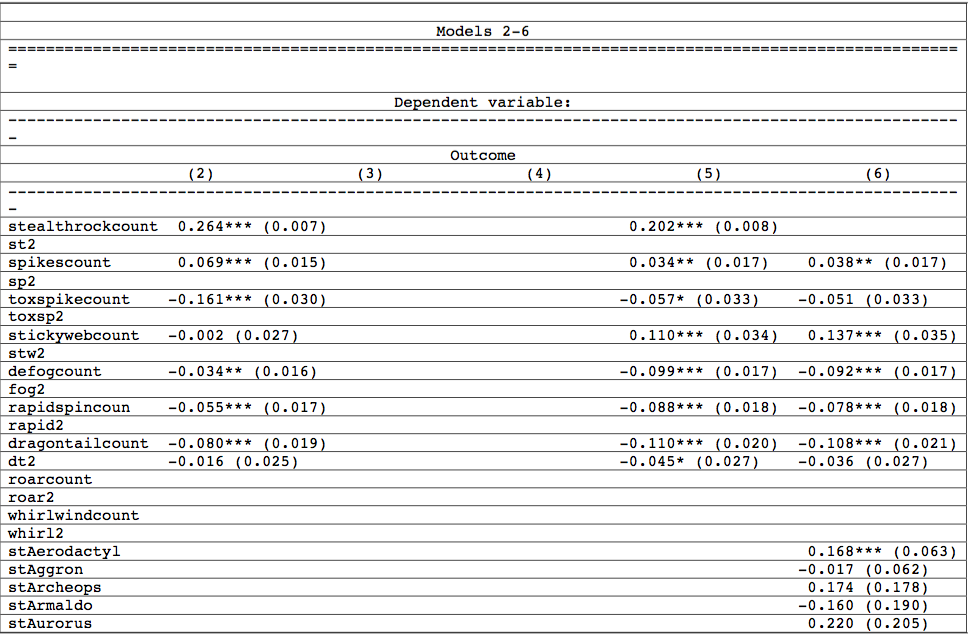
\includegraphics[width=400px]{m1} \end{center}
  
  \begin{center}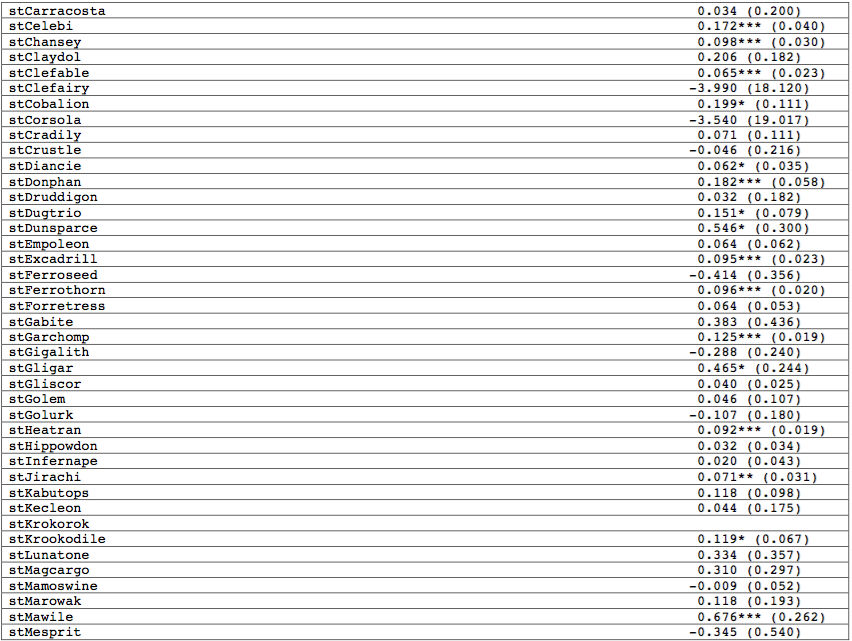
\includegraphics[width=400px]{m2} \end{center}
  
  \begin{center}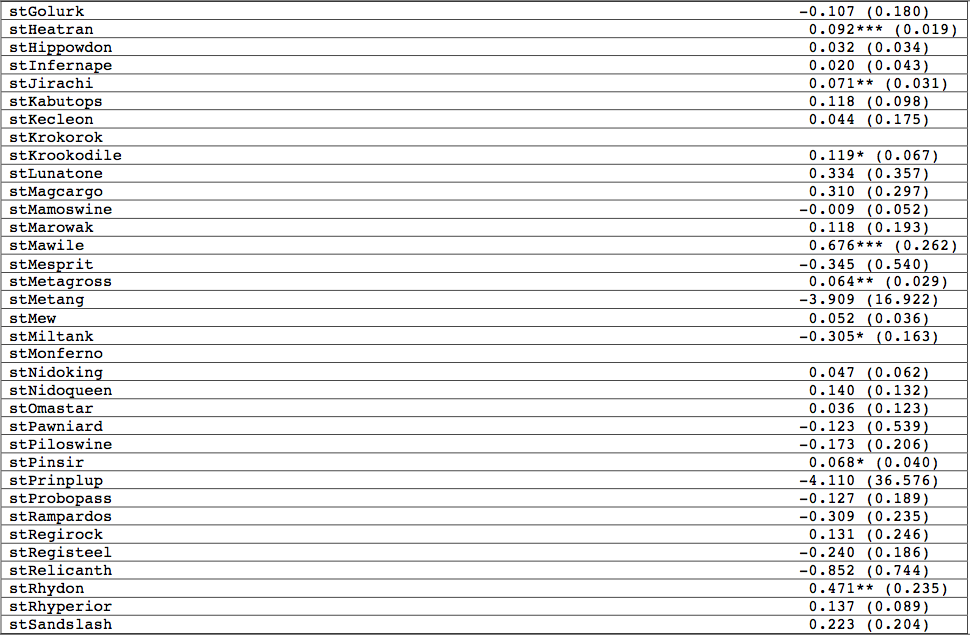
\includegraphics[width=400px]{m3} \end{center}
  
  \begin{center}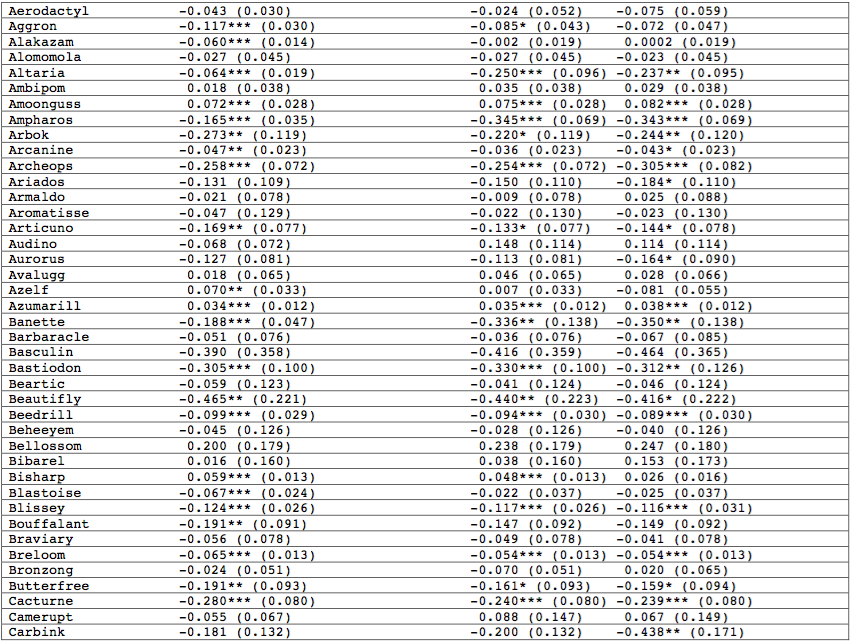
\includegraphics[width=400px]{m4} \end{center}
  
  \begin{center}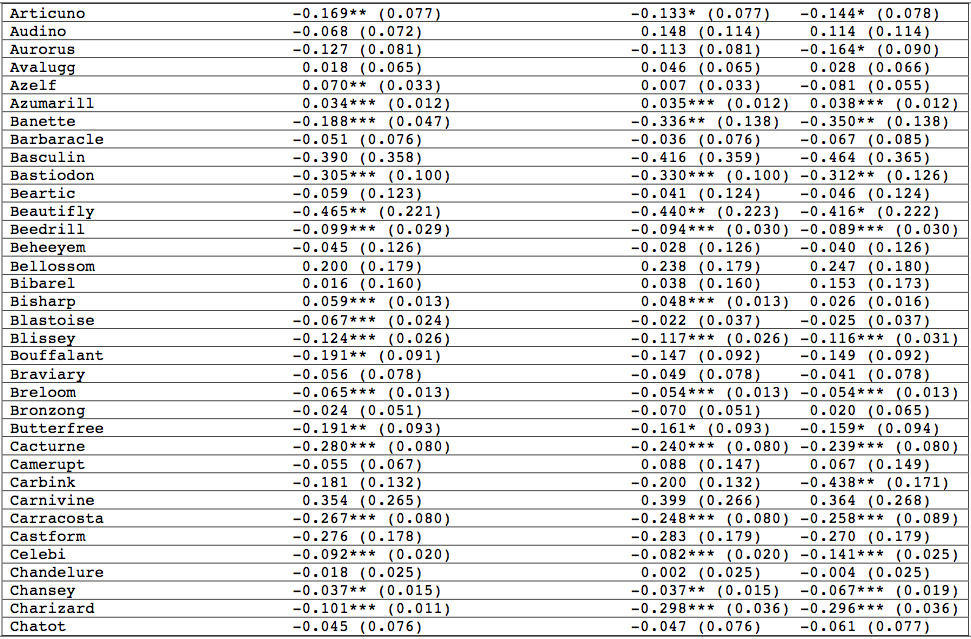
\includegraphics[width=400px]{m5} \end{center}
  
  \begin{center}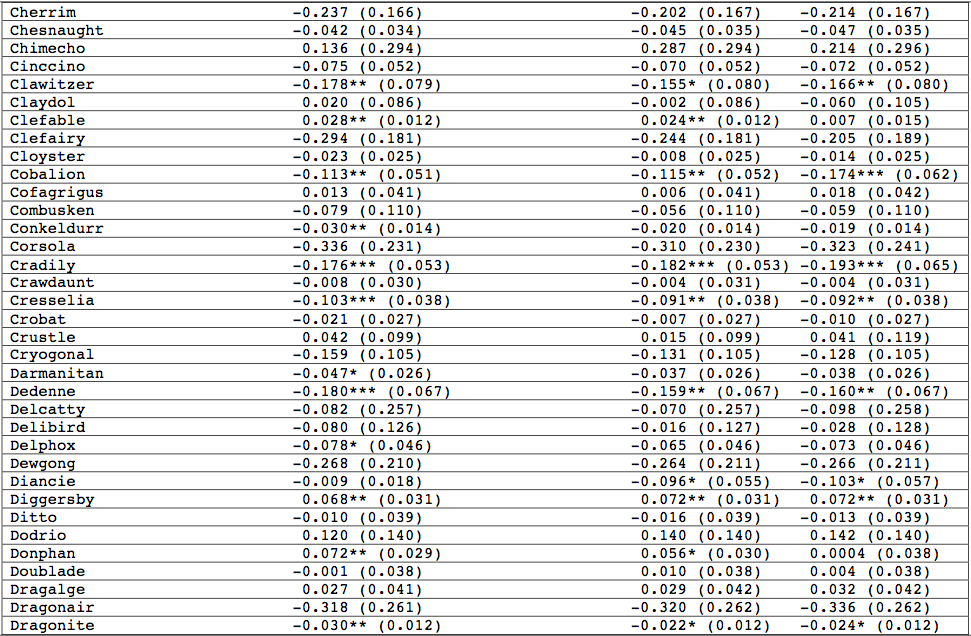
\includegraphics[width=400px]{m6} \end{center}
  
  \begin{center}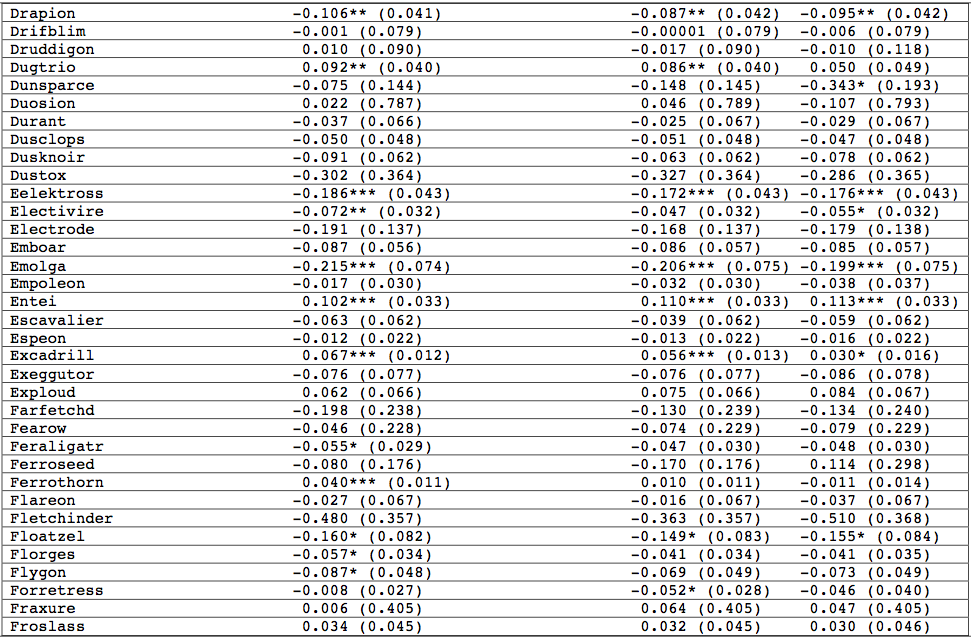
\includegraphics[width=400px]{m7} \end{center}
  
  \begin{center}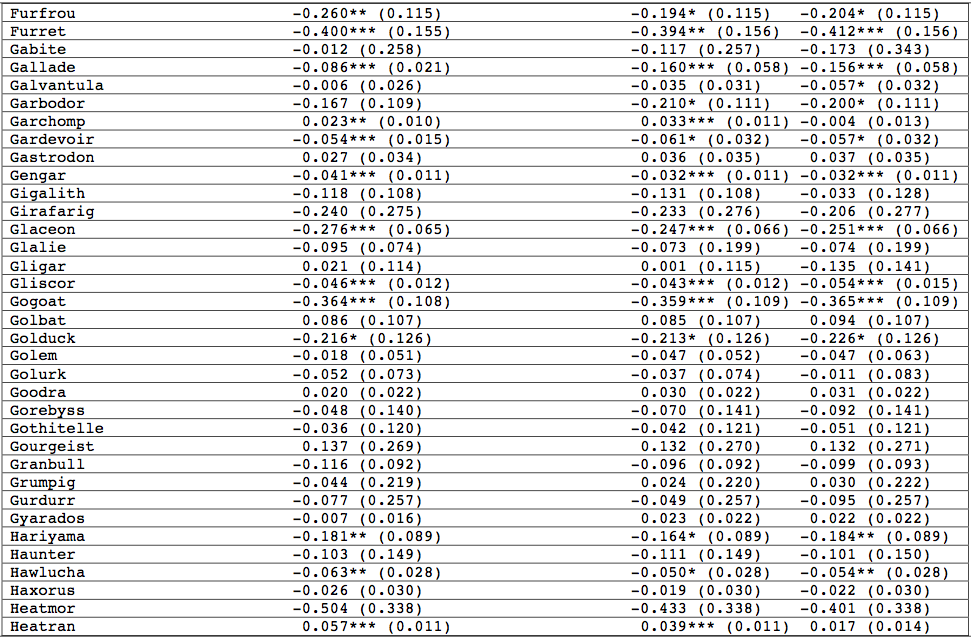
\includegraphics[width=400px]{m8} \end{center}
  
  \begin{center}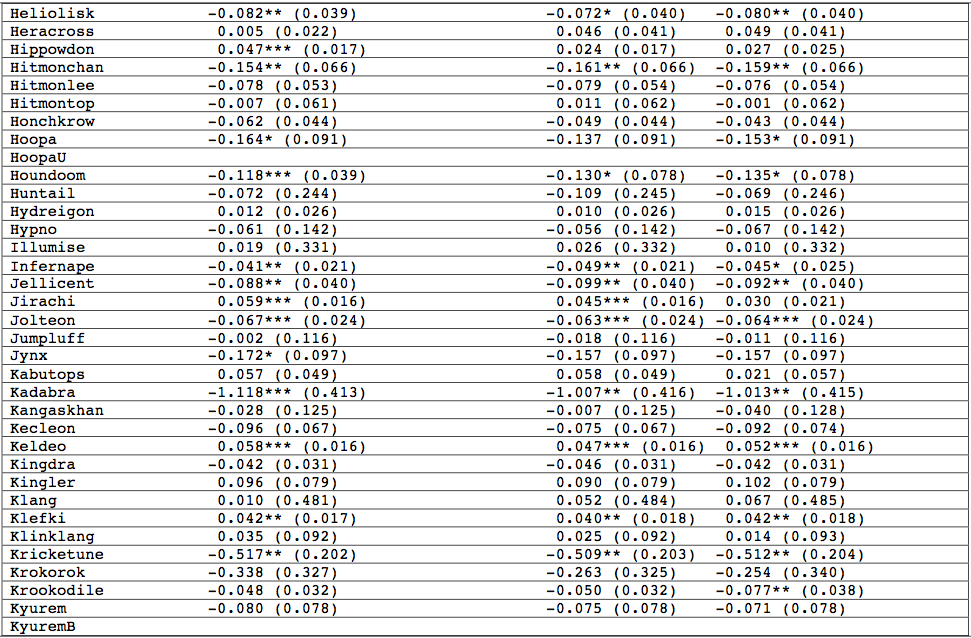
\includegraphics[width=400px]{m9} \end{center}
  
  \begin{center}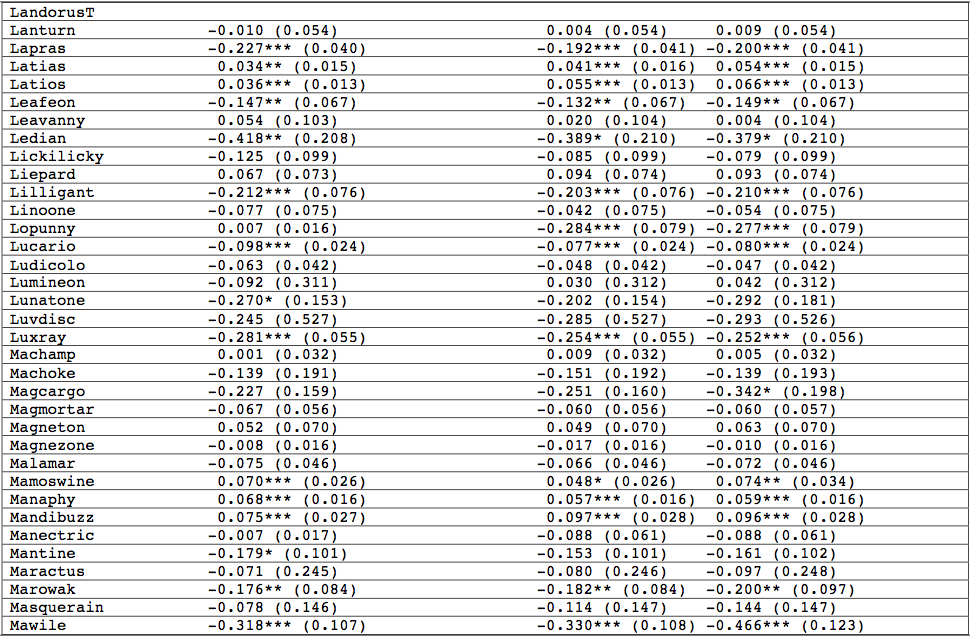
\includegraphics[width=400px]{m10} \end{center}
  
  \begin{center}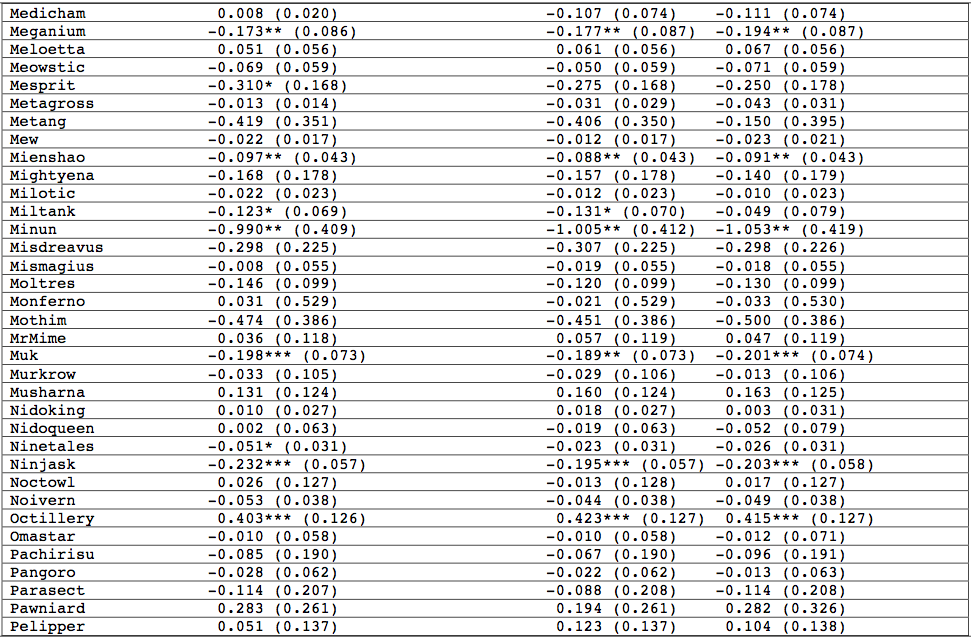
\includegraphics[width=400px]{m11} \end{center}
  
  \begin{center}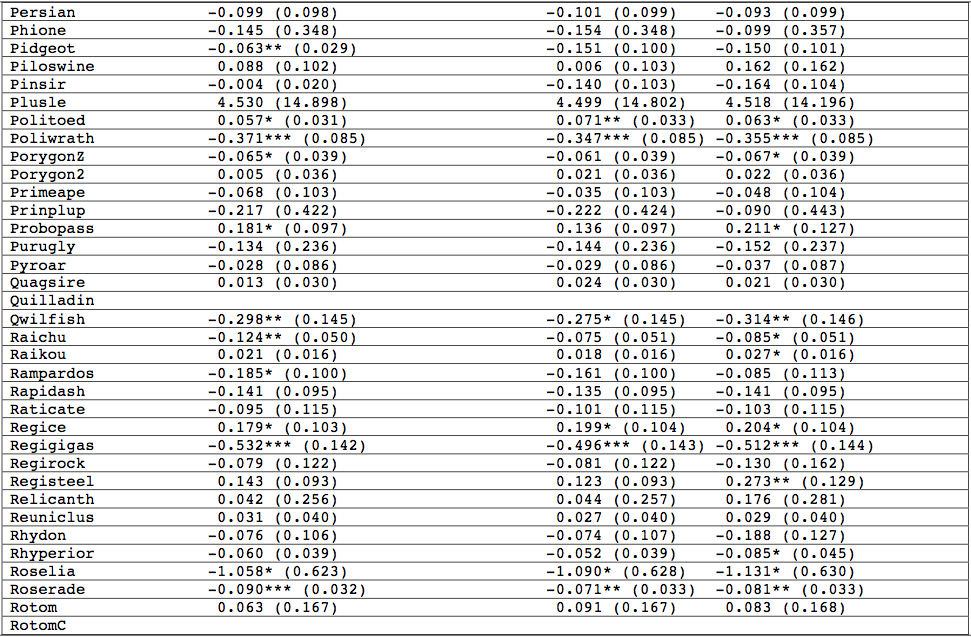
\includegraphics[width=400px]{m12} \end{center}
  
  \begin{center}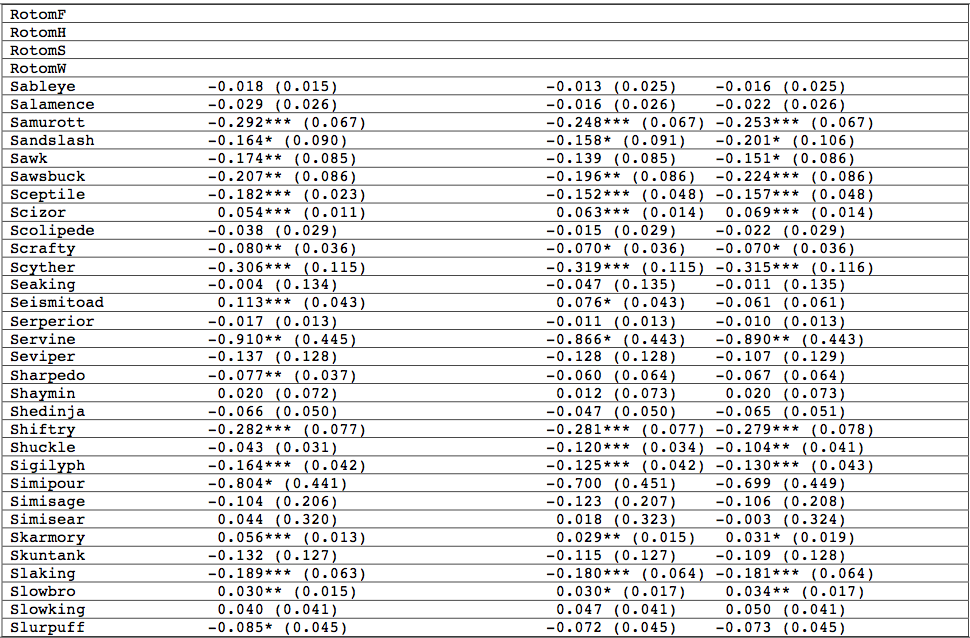
\includegraphics[width=400px]{m13} \end{center}
  
  \begin{center}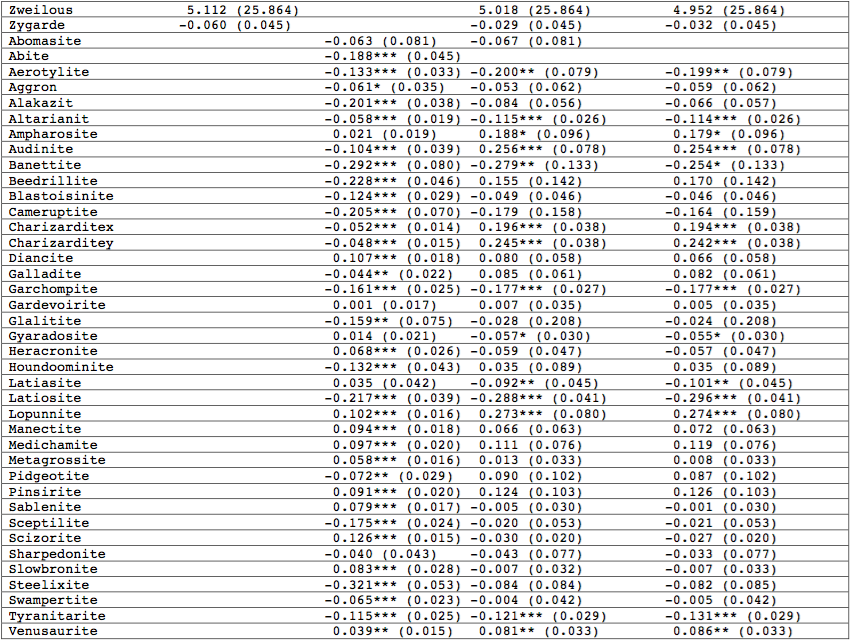
\includegraphics[width=400px]{m14} \end{center}
  
  \begin{center}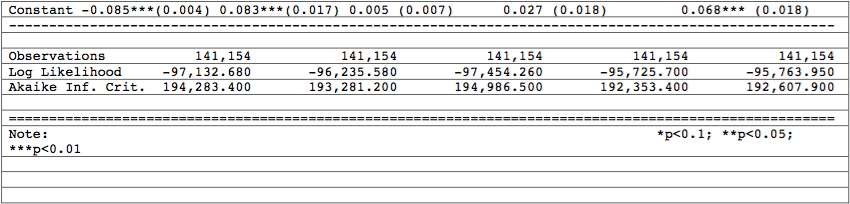
\includegraphics[width=400px]{m15} \end{center}
  
  \textbf{In the main Rmd file}
  
  \begin{Shaded}
  \begin{Highlighting}[]
  \CommentTok{# This chunk ensures that the thesisdown package is}
  \CommentTok{# installed and loaded. This thesisdown package includes}
  \CommentTok{# the template files for the thesis.}
  \NormalTok{if(!}\KeywordTok{require}\NormalTok{(devtools))}
    \KeywordTok{install.packages}\NormalTok{(}\StringTok{"devtools"}\NormalTok{, }\DataTypeTok{repos =} \StringTok{"http://cran.rstudio.com"}\NormalTok{)}
  \NormalTok{if(!}\KeywordTok{require}\NormalTok{(thesisdown))}
    \NormalTok{devtools::}\KeywordTok{install_github}\NormalTok{(}\StringTok{"ismayc/thesisdown"}\NormalTok{)}
  \KeywordTok{library}\NormalTok{(thesisdown)}
  \end{Highlighting}
  \end{Shaded}
  
  \textbf{In Chapter \ref{ref-labels}:}
  
  \begin{Shaded}
  \begin{Highlighting}[]
  \CommentTok{# This chunk ensures that the thesisdown package is}
  \CommentTok{# installed and loaded. This thesisdown package includes}
  \CommentTok{# the template files for the thesis and also two functions}
  \CommentTok{# used for labeling and referencing}
  \NormalTok{if(!}\KeywordTok{require}\NormalTok{(devtools))}
    \KeywordTok{install.packages}\NormalTok{(}\StringTok{"devtools"}\NormalTok{, }\DataTypeTok{repos =} \StringTok{"http://cran.rstudio.com"}\NormalTok{)}
  \NormalTok{if(!}\KeywordTok{require}\NormalTok{(dplyr))}
      \KeywordTok{install.packages}\NormalTok{(}\StringTok{"dplyr"}\NormalTok{, }\DataTypeTok{repos =} \StringTok{"http://cran.rstudio.com"}\NormalTok{)}
  \NormalTok{if(!}\KeywordTok{require}\NormalTok{(ggplot2))}
      \KeywordTok{install.packages}\NormalTok{(}\StringTok{"ggplot2"}\NormalTok{, }\DataTypeTok{repos =} \StringTok{"http://cran.rstudio.com"}\NormalTok{)}
  \NormalTok{if(!}\KeywordTok{require}\NormalTok{(ggplot2))}
      \KeywordTok{install.packages}\NormalTok{(}\StringTok{"bookdown"}\NormalTok{, }\DataTypeTok{repos =} \StringTok{"http://cran.rstudio.com"}\NormalTok{)}
  \NormalTok{if(!}\KeywordTok{require}\NormalTok{(thesisdown))\{}
    \KeywordTok{library}\NormalTok{(devtools)}
    \NormalTok{devtools::}\KeywordTok{install_github}\NormalTok{(}\StringTok{"ismayc/thesisdown"}\NormalTok{)}
    \NormalTok{\}}
  \KeywordTok{library}\NormalTok{(thesisdown)}
  \KeywordTok{load}\NormalTok{(}\StringTok{"data/d1.Rda"}\NormalTok{)}
  \end{Highlighting}
  \end{Shaded}
  
  \backmatter
  
  \chapter{References}\label{references}
  
  \begin{itemize}
  \tightlist
  \item
    Ariely, D. (2009). Predictably irrational: The hidden forces that
    shape our decisions. New York, NY: Harper. Chapter 8: Keeping Doors
    Open (pp.~139-154).
  \item
    Ho, H., Ramesh, V. (2016) Percymon: A Pokemon Showdown Artifical
    Intelligence. Retrieved October 31, 2016, from:
    \url{http://robots.stanford.edu/cs221/2016/restricted/projects/vramesh2/final.pdf}
  \item
    Pokémon Company International (Nov. 21, 2014) Pokémon Omega Ruby \&
    Pokémon Alpha Sapphire: The Official Hoenn Region Strategy Guide.
  \item
    Pokémon Showdown! battle simulator (n.d.). Retrieved October 31, 2016,
    from \url{http://pokemonshowdown.com/}
  \item
    Pokémon Showdown Github Master Repository (2016).
    Zarel/Pokemon-Showdown. Retrieved October 31, 2016, from
    \url{https://github.com/Zarel/Pokemon-Showdown/tree/master/data}
  \item
    Sanchez-Ante, Gildardo (Dec., 2013) Sistemas Inteligentes: Reportes
    Finales Ago-Dic 2013. Retrieved October 31, 2016, from:
    \url{https://www.researchgate.net/profile/Gildardo_Sanchez-Ante/publication/259343975_Sistemas_Inteligentes_Reportes_Finales_Ago-Dic_2013/links/0c96052b1d0b582e95000000.pdf\#page=140}
  \item
    Schwalbe, U., \& Walker, P. (2001). Zermelo and the Early History of
    Game Theory. Games and Economic Behavior, 34(1), 123-137.
    \url{doi:10.1006/game.2000.0794}
  \item
    Smogon University (n.d.). Retrieved October 31, 2016, from
    \url{http://www.smogon.com/}
  \item
    Wunder, M., Kaisers, M., Yaros, J., Littman, M., (May, 2011) Using
    Iterated Reasoning to Predict Opponent Strategies. Proc. of 10th Int.
    Conf. on Autonomous Agents and Multiagent Systems (AAMAS 2011), Tumer,
    Yolum, Sonenberg and Stone (eds.), 593-600. --\textgreater{} \noindent
  \end{itemize}
  
  \setlength{\parindent}{-0.20in} \setlength{\leftskip}{0.20in}
  \setlength{\parskip}{8pt}
  
  \begin{center}\rule{0.5\linewidth}{\linethickness}\end{center}


  % Index?

\end{document}

